%\documentclass[conference]{IEEEtran}
\documentclass[10pt,conference,anonymous]{IEEEtran}
\IEEEoverridecommandlockouts

%% Marcelo added this
\makeatletter
\renewcommand\footnoterule{%
  \kern-3\p@
  \hrule\@width.4\columnwidth
  \kern2.6\p@}
  \makeatother




\usepackage{inconsolata}
\usepackage{listings}

\lstset{language=Java,
basicstyle=\ttfamily\scriptsize,
%basicstyle=\ttfamily,
keywordstyle=\color{javapurple}\bfseries,
stringstyle=\color{pblue},
commentstyle=\color{javagreen},
morecomment=[s][\color{javadocblue}]{/**}{*/},
morecomment=[s][\color{gray}]{@}{\ },
numbers=left,
numberstyle=\tiny\color{black},
stepnumber=2,
numbersep=8pt,
tabsize=4,
showspaces=false,
showstringspaces=false,
breaklines=true,}

%%%%%%%%%%%%%%%%%%%%%%%%%%%%%%%%%%




\usepackage{adjustbox} % ajustar tabela ao tamanho da pagina

\usepackage{tikz}
\usetikzlibrary{matrix,fit,shapes,calc,positioning,shadows,arrows,shapes,backgrounds,decorations.markings,fadings}
\usepackage{graphicx}
\usepackage{multirow}
\usepackage[caption=false, font=footnotesize]{subfig}
\usepackage{wrapfig}
\usepackage{enumitem}
\usepackage{url}
%% helpers
\newcommand{\js}{JS}
\newcommand{\javascript}{JavaScript}
\newcommand{\es}{ES}
\newcommand{\ecmascript}{\es{}}
\newcommand{\tname}{TNAME}
\newcommand{\Comment}[1]{}
\newcommand{\numsubjects}{5}
\newcommand{\etal}{and colleagues'}
\newcommand{\ie}{i.e.}
\newcommand{\eg}{e.g.}
\newcommand{\cmark}{\ding{51}}%
\newcommand{\xmark}{{\color{red}\ding{55}}}%
\newcommand{\pGoodGood}{$\mathit{P}${\small\cmark\!\cmark}}%
\newcommand{\pGoodBad}{$\mathit{P}${\small\cmark\!\xmark}}%
\newcommand{\pBadDontCare}{$\mathit{P_?}$}%
\newcommand{\sfl}{SFL\xspace}
\newcommand{\ddg}{DDG\xspace}
\newcommand{\totfiles}{$\sim$38K}

%% annotations
\newif\ifdraftmode
%% Comment or uncomment the \draftmodetrue line.
\draftmodetrue
\ifdraftmode
 \newcommand{\Fix}[1]{\textbf{[[}{\color{red} #1}\textbf{]]}}
 \newcommand{\Mar}[1]{\textbf{[[Marcelo: }{\color{magenta} #1}\textbf{]]}}
 \newcommand{\Igor}[1]{\textbf{[[Igor: }{\color{blue} #1}\textbf{]]}}
 \newcommand{\note}[1]{\todo[inline,color=red!30,caption={}]{#1}}
\else
 \newcommand{\Fix}[1]{\relax}
 \newcommand{\Mar}[1]{\relax}
 \newcommand{\Igor}[1]{\relax}
 \newcommand{\note}[1]{\relax}
\fi

% For submitted version only.
\pagenumbering{arabic}

% Uncomment this if you need more space
%% \makeatletter
%% \def\@copyrightspace{\enlargethispage{-10pt}\relax}
%% \makeatother

\newcommand{\codesize}{\small}
\newcommand{\CodeIn}[1]{\mcodeid{#1}}
\newcommand{\CodeInM}[1]{\mcodeid{#1}}
% \|name| or \mathid{name} denotes identifiers and slots in formulas
\def\|#1|{\mathid{#1}}
\newcommand{\mathid}[1]{\ensuremath{\mathit{#1}}}
% \<name> or \codeid{name} denotes computer code identifiers
\def\<#1>{\codeid{#1}}
\newcommand{\codeid}[1]{\ifmmode{\mbox{\codesize\ttfamily{#1}}}\else{\codesize\ttfamily #1}\fi}
\def\<#1>{\mcodeid{#1}}
\newcommand{\mcodeid}[1]{\mbox{\codesize\ttfamily{#1}}}

%% thumbs up down
\newcommand*{\RightThumbsUpAux}[1]{%
  \begingroup
    \sbox0{Ag}%
    \raisebox{-\dp0}{%
      \includegraphics[{%
        height=\dimexpr\dp0+\ht0\relax,
        #1%
      }]{thumbsup.pdf}%
    }%
  \endgroup
}
\newcommand*{\RightThumbsUp}{%
  \RightThumbsUpAux{}%
}
\newcommand*{\RightThumbsDown}{%
  \RightThumbsUpAux{origin=c,angle=180}%
}
\newcommand*{\LeftThumbsUp}{%
  \scalebox{-1}[1]{\RightThumbsUp}%
}
\newcommand*{\LeftThumbsDown}{%
  \scalebox{-1}[1]{\RightThumbsDown}%
}

\newcommand{\checkm}{Y}
\newcommand{\crossmark}{N}
%\begin{wraptable}[20]{t}[0pt]{0.5\textwidth}

\newcommand{\totalTestFiles}{38,369}
\newcommand{\totalTestFilesCompileInAll}{35,939}
\newcommand{\totalTestFilesPassInAll}{24,493}
\newcommand{\nofuzzAll}{209}
\newcommand{\nofuzzBugs}{\Fix{XX}}
\newcommand{\nofuzzDuplicates}{63}
\newcommand{\nofuzzFalsePositives}{24}
\newcommand{\nofuzzHITotal}{177}
\newcommand{\nofuzzLOTotal}{32}
\newcommand{\nofuzzTotalFiles}{977} % conflicting files
\newcommand{\nofuzzFilesHI}{940} % conflicting files HI
\newcommand{\nofuzzFilesLO}{37} % conflicting files LO

\newcommand{\nofuzzBucketsBugsHI}{\Fix{124}} % buckets reported (including dups)
\newcommand{\nofuzzBucketsBugsLO}{\Fix{11}} % buckets reported
\newcommand{\nofuzzDupsHI}{\Fix{X}}
\newcommand{\nofuzzDupsLO}{\Fix{Y}}

% continue updating bugs table
\newcommand{\tableBugsNum}{\Fix{26}}

%% anonymize

\newcommand{\anonym}[1]{{\tiny\colorbox{black}{#1}}}

%% names
\newcommand{\radamsa}{radamsa}
\newcommand{\quickfuzz}{quickfuzz}

\newcommand{\jsc}{JavaScriptCore}
\newcommand{\veight}{V8}
\newcommand{\chakra}{Chakra}
\newcommand{\smonkey}{SpiderMonkey}
\newcommand{\jerry}{JerryScript}

\newcommand{\lo}{lo}
\newcommand{\hi}{hi}


\begin{document}

%Should I Fuzz my Inputs or Improve my Tests? 
\title{Leveraging Diversity to Find Bugs\\ in JavaScript Engines}

%% \author{
%% \IEEEauthorblockN{Sabrina Souto}
%% \IEEEauthorblockA{State University of Para\'iba\\
%% Para\'iba, Brazil\\
%% sabrinadfs@gmail.com}
%% \and
%% \IEEEauthorblockN{Marcelo d'Amorim}
%% \IEEEauthorblockA{Federal University of Pernambuco\\
%%   Pernambuco, Brazil\\
%%   damorim@cin.ufpe.br}
%% \and
%% \IEEEauthorblockN{Rohit Gheyi}
%% \IEEEauthorblockA{Federal University of Campina Grande\\
%%   Para\'iba, Brazil\\
%%   rohit@dsc.ufcg.edu.br}
%% }

\maketitle

%% page numbering -M
\thispagestyle{plain}
\pagestyle{plain}

%% JavaScript (\js{}) is a popular programming language for the
%% web. Finding errors in JS runtime engines is an important problem.
\begin{abstract}
JavaScript is a very popular programming language today, permeating
different domains of application. Several JavaScript engines compete
for dominance and bugs on these engines are not rare. One important
reason for that is the language specification, which is incomplete and
evolves frequently.

This paper reports on a study to assess reliability
of JavaScript engines by leveraging the rich diversity of open-source
implementations. For that, we explored two methods---test
transplantation and cross-engine differential testing. Test
transplantation evaluates the effects of running test suites of a given
engine in another engine. Cross-engine differential testing evaluates
the effects of fuzzing existing inputs and then comparing the output
produced by different engines with a differential oracle.

Our results indicate that \Fix{...}
\end{abstract}

\begin{IEEEkeywords}
JavaScript; Diversity; Software Testing
\end{IEEEkeywords}

\section{Introduction}

JavaScript (\js{}) is today one of the most popular programming
languages around~\cite{business-insider,stackify}, with significant
penetration in various segments including, web development, mobile,
and, more recently, the Internet of
Things~(IoT)~\cite{simply-technologies}. The interest of the community
for the language encourages constant improvements in its specification
and implementations. It is natural to expect that such improvements
lead to sensible implementation changes. Even small changes can have
high practical impact. For example, in October 2014 a new attribute
added to Array objects resulted in the MS Outlook Calendar web app
stop working under
Chrome~\cite{array-bug-chromium-issue4247,array-bug-discussion}.
Intuitively, developing reliable engines is difficult because
specifications are incomplete and evolve frequently.


Finding bugs in \js\ engines is an important problem given the range
of applications that could be affected with those
bugs. It\Comment{Finding bugs in \js\ engines} is also
challenging. For example, a test that passes in one engine could
legitimately fail in a different engine because of some undefined
behavior in the spec\footnote{These cases of undefined behavior can be
  localized by searching for the string ``implementation-dependent''
  in the ES6 spec document~\cite{ecmas262-spec}.}. As another example,
a test may fail because the engine does not fully implement some
feature. The publicly-available Kangax compatibility
table~\cite{kangax} relates features of \js\ with the engines that
support them. To sum, it is often non-trivial to assess if a test
fails because of a bug or because of some other reason making test
automation more challenging.

%% when a bug is found in some engine a test case is created and added to
%% the regression suite. Those test inputs often check interesting
%% scenarios that could reveal bugs in different engine
%% implementations. 

%% WHAT WE DID
The goal of this paper is to assess reliability of popular
\js\ engines. The paper reports the results of a study that evaluates
the effectiveness of two complementary diversity-aware testing techniques. \emph{Test transplantation} leverages
diversity of test cases to find bugs. It evaluates the effects that
running \js{} test files from a given engine have in detecting bugs in
other engines. The intuition is that developers design test cases
differently; hence replaying the test in a different engine may reveal
unanticipated problems. \emph{Cross-engine differential testing}
evaluates the ability of leveraging diversity of engine
implementations to find bugs. More precisely, it fuzzes existing test
inputs~\cite{fuzz-testing-history} and then compares the output
produced by different engines using a differential oracle. One of
various causes of output discrepancy is a bug. It is worth noting that
Differential Testing~\cite{Brumley-etal-ss07} (DT) has been applied in
a variety of contexts to find
bugs~\cite{Yang-etal-pldi11,Chen-etal-fse2015,Argyros-etla-ccs16,Chen-etal-pldi16,petsios-etal-sp2017,SivakornAPKJ17,Zhang:2017:ATD:3097368.3097448}. It
automates test generation in scenarios where multiple implementations
of a system exist. DT leverages the diversity across system's
implementations to detect anomalous behavior. For example, Mozilla
runs JS files\footnote{These files are created with the grammar-based fuzzer
  jsfunfuzz~\cite{jsfunfuzz}. Look for option ``compare\_jit'' from funfuzz.} against different configurations of their
\smonkey{} engine~\cite{jsfunfuzz-mozilla-bug} to find discrepancies
across different configurations of the same build (\eg{}, enabling or
not eager JIT compilation). They use this technique since 2002 and
have been able to find over 270 bugs since
then~\cite{jsfunfuzz-at-mozilla}, including security bugs.  In
contrast, cross-engine differential testing--the technique used in
this work--checks functional correctness by comparing the output
produced by \emph{different engines} on a fuzzed
input~\cite{patra2016learning} as opposed to different builds of the
same engine. This approach has not been
popularized, certainly, because it is still not practical to fully automate--a
number of legitimate reasons exist, other than a bug, for a test
execution to manifest discrepancy (see
Table~\ref{tab:false-positives}). This study quantifies human effort
to find these bugs using this method.

%% WHAT WE FOUND
To sum, we found that \Fix{...}

%% LIST OF CONTRIBUTIONS
This paper makes the following contributions \Fix{...}

\section{JavaScript}
\label{sec:es6-design}
\label{sec:imp-dep-behavior}

JavaScript engines are virtual machines that parse source code,
compile it in bytecodes, and run these bytecodes. These engines
implement some version of the ECMAScript (\es{}), which emerged with
the goal to standardize variants of the language, such as Netscape's
JavaScript and Microsoft's JScript\footnote{The name JavaScript still
  prevails today, certainly for historical reasons.}. The \es{}
specification is regulated by Ecma International~\cite{es6-website}
under the TC39~\cite{tc39-github} technical committee.  Every year, a
new version of the \es{} specification is produced with new features
and minor fixes. The canonical spec today is
ES6~\cite{ecmas262-spec-repo,ecmas262-spec}.

%% In the following, we briefly describe different sources of
%% discrepancies that can emerge across different engine implementations
%% as results of the active changes in the \es{} specification.
%% .........
%% A compatibility table relating features and supporting engines is
%% publicly available~\cite{kangax}.

Both the specification and implementation of JavaScript are
incomplete. Certain parts of the specification are undefined; it is
responsibility of engine engineers to decide how to implement these
functionalities. The JavaScript spec uses the label
``implementation-dependent'' to indicate these cases, where behavior
may differ from engine to engine. One reason this flexibility in the
spec exists is to enable compiler optimizations. For example, the
\mcodeid{for-in} loop does not clearly specify the iteration
order~\cite{so-forin-undefined,javascript-in-chrome} and different
engines capitalize on that~\cite{for-in-undefined}.  As another
example, the latest version of the \es{} specification states that if
the \mcodeid{Number.toPrecision()} function is called with more than
one argument, then the behavior is
implementation-dependent~\cite{es6-toPrecision}. Various other cases
like these exist in the specification. Such gap also exists at the
implementation level. Given the speed the specification changes and
the complexity of the language some features are not fully implemented
as can be observed by the Kangax compatibility table~\cite{kangax}.

\sloppy It is also worth noting that, as in other languages, some
elements in JS have non-deterministic behavior (\eg{},
\mcodeid{Math.random} and \mcodeid{Date}). A test that make decisions
based on these elements could, in principle, produce different
outcomes on different runs. Carefully-written test cases should not
manifest this kind of
flakiness~\cite{luo-etal-fse2014,palomba-zaidman-icsme2017}, but
fuzzed test files could are more likely, intuitively, to manifest
them.

As mentioned previously, all those aspects make testing \js\ engines
more challenging.


%\subsection{Randomness}


%\subsection{\Fix{Other}}

%% 1) The stack depth in JS is often close to the real (native) C stack
%% depth, nevertheless observable by JS through recursion. This causes
%% differential behavior even on the same engine when JITs are enabled or
%% disabled, as the stack frame sizes vary. LangFuzz in particular
%% produces a lot of recursions and hits these problems even more often
%% than jsfunfuzz.\Mar{ask C. Holler. it is unclear to me how the output
%%   could be different.}

\section{Objects of Study}
\label{sec:methodology}

This section discusses the objects we used in our study.

\subsection{Engines}
\label{sec:methodology:engines}~We selected 
JS engines according to the following criteria.

\begin{itemize}
\item Released latest version after Jan 1, 2018
\item Contains more than 1K starts, if on GitHub  
\item Uses a public issue tracker
\end{itemize}  

We look for highly-maintained (as per the first criterion) and popular
(as per the second criterion) projects. As we wanted to report bugs,
we also looked for project with public issue
trackers. Table~\ref{tab:engines} lists the engines we analyzed in
this work. It is worth noting that we used GoogleChromeLab's JSVU
tool~\cite{jsvu} to automatically install and configure versions of
different JS engines in our host environment. This is important as we
aim to use the most recent stable versions of each engine as to avoid
reporting old and already-fixed bugs to developers.

%% Table~\ref{tab:engines} shows the engines we selected in this
%% study. We made an exception to the second criterion with
%% XS~\cite{xs2018repo}. As the project is young, created in Oct 2017, we
%% thought there was insufficient time to obtain 1K stars for XS. We
%% still considered this project as it seems to be attracting interest
%% from the community\Fix{is this true?}

\begin{table}[t]
  \centering
  \caption{\label{tab:engines}Engines analyzed.}
  \begin{tabular}{cccr}
    \toprule
    Team & Name & URL & \# Stars \\
    \midrule
    Apple & \jsc{} (WebKit) & \cite{jsc2018repo} & \multicolumn{1}{c}{3300+} \\
    Google & \veight{} & \cite{v82018repo} & 9800+ \\
%    \jerry{} & \jerry{} & \cite{jerryscript2018repo} & 3100+ \\
    Microsoft & \chakra{} & \cite{chakra2018repo} & 7200+ \\
%    Moddable & XS & \cite{xs2018repo} & 140+ \\
    %% \midrule
    %% \multirow{2}{*}{Mozilla} & Rhino & \cite{rhino2018repo} & 1800+ \\
    Mozilla & \smonkey{} & \cite{spidermonkey2018repo} & \multicolumn{1}{c}{1100+} \\
   \bottomrule     
  \end{tabular}
\end{table}

\subsection{Seed JS files\label{sec:seeds}}~
We selected test files from several public projects from GitHub. We
looked for self-contained tests from JS engine projects, initially
using the GitHub REST API~\cite{github-rest-api}. We noticed that some
of the tests we found depend on external libraries, which not all
engines we use support. We decided to discard those. For example, many
tests we found required a Node.js runtime~\cite{node} for
execution. The main source of test cases is the official
Test262~\cite{tc39-github} conformance test suite for the ECMA262
specification~\cite{ecmas262-spec}. This test suite contains 87\% of
all the tests we used. We also considered test suites of three of the
four engines mentioned in Section~\ref{sec:methodology:engines} and
four other engines. Table~\ref{tab:test-suites} shows the breakdown of
tests we considered. Column ``original'' shows the test cases for each
test suite. Overall, we found a total of \totfiles{} JS files. We did
not consider tests from the \chakra{} repository because they depend
on non-portable objects. Notice that the number of tests in
\veight\ is low. That happens because many tests in \veight{} are
inherited from Mozilla and \jsc{}; we discarded those to avoid
repetition and to give credit where it is due. Column
``compile-in-all'' shows the number of test cases for which all four
engines we analyzed do not throw compile-time error. We discarded
tests that manifest compile errors as they clearly indicate missing
features; these tests use non-portable names (\eg{}, \jsc{}'s
\CodeIn{drainMicrotasks()} and \smonkey{}'s \CodeIn{Error.lineNumber})
or use functions that, although being part of the spec, not all
engines currently support. Finally, column ``no-fail-in-all'' shows
the tests for which all engines
pass. Section~\ref{sec:transplantation} discusses these failures, some
of which are indicative of bugs. The tests under this column will be
used to create new, potentially fault-revealing, tests. For that, it
is important to assure that all of them pass.

It is also worth mentioning that some engines use a custom shell to
run tests, including a harness with specific assertions.  For these,
we needed to make small changes in the testing infrastructure to be
able to run the tests uniformly across all engines. More precisely, we
needed to mock non-portable harness functions, which are only
available to certain engines.

 %% The table shows the
 %%    number of test cases in each test suite considered: TC-39
 %%    conformance test suite, suites from engines we analyzed, and
 %%    suites from other engines.

\begin{table}[t]
  \centering
  \caption{\label{tab:test-suites}Number of test cases per
    suite. Column ``original'' shows the original size of the test
    suite, column ``compile-in-all'' shows the number of test cases
    for which engines do not throw compile error (\eg{}, undefined
    name), and column ``no-fail-all'' shows the number of test cases
    that pass in all four engines we analyzed.}
  \begin{tabular}{ccrrr}
    \toprule
    \multirow{2}{*}{Name}      &  \multirow{2}{*}{Source} &
    \multicolumn{3}{c}{\# JS files} \\
    \cline{3-5}
                               &         & original & compile-in-all &  no-fail-in-all \\
    \midrule
    TC-39 (Test262) & \cite{ecma262-conformance-suite} & 31,276 &
    29,846 & 18,943 \\
    \midrule
    \jsc{} & \cite{webkit} & 1,031 & 1,021 & 955\\
    \smonkey\ & \cite{mozilla} & 2,634 & 2,116 & 1,686\\
    \veight{} & \cite{v8} & 75 & 57 & 57\\
    \midrule
    Duktape & \cite{duktape} & 1,195 & 921 & 915\\ 
    \jerry{} & \cite{jerryscript} & 1,951 & 1,878 & 1,837\\
    JSI & \cite{jsi} & 99 & 63 & 63\\
    Tiny-js & \cite{tinyjs} & 49 & 37 & 37\\
    % \chakra{} & \cite{chakracore} & 2632 \\
    \midrule
     &  & \totalTestFiles{} & \totalTestFilesCompileInAll{} & \totalTestFilesPassInAll{}\\
   \bottomrule 
  \end{tabular}
\end{table}

% For example to run the \jerry{} tests it was necessary 
% use the unit-test package to run it, but with our changes we added the assertion
% does not have an assertion in the test file
% \Fix{add code to explain}

\subsection{Fuzzers}
\label{sec:objects:fuzzers}

%% In the following, we describe the list of fuzzers we analyzed. We
%% initially considered generational grammar-based fuzzers and mutational
%% fuzzers.

Fuzzers are typically categorized in two main groups--those that build
inputs anew (generational) and those that modify existing inputs
(mutational). We used two black-box mutational
fuzzers\Comment{Radamsa~\cite{radamsa} and QuickFuzz~\cite{quickfuzz}}
in this study. In the following, we provide rationale for this
selection.

Generational fuzzers are typically grammar-based. These fuzzers
generate a new file using the grammar of the language whose inputs
should be fuzzed. Intuitively, those fuzzers implement a traversal of
the production rules of the input grammar to create syntax trees,
which are then pretty-printed. Consequently, this approach produces
inputs that are syntactically valid by construction. We analyzed four
grammar-based fuzzers--Grammarinator~\cite{grammarinator},
jsfunfuzz~\cite{jsfunfuzz},
LangFuzz~\cite{Holler:2012:FCF:2362793.2362831}, and
Megadeth~\cite{grieco2016quickfuzz}.  Unfortunately, none of those
were effective out of the box. For example, we produced 100K inputs
with Grammarinator and only \Fix{X} of those were valid. With
Megadeth, we were able to produce \Fix{Y, Y$>$Y?}  valid inputs as it
contains some heuristics to circumvent violations of certain type
rules such as \Fix{variable used must be defined?}. Nonetheless,
running those inputs in our infrastructure we were unable to find
discrepancies. Inspecting those inputs, we realized that they reflected
very simple scenarios. To sum, a high percentage of inputs that
Grammarinator and Megadeth generated were semantically-invalid that we
needed to discard whereas the valid inputs manifested no
discrepancies. Considering jsfunfuzz~\cite{jsfunfuzz}, we noticed
that, in addition to the issues mentioned above, it produces inputs
that use functions that are only available in the \smonkey{}
engine. We would need either to mock those functions in other engines
or to discard those tests. Considering
LangFuzz~\cite{Holler:2012:FCF:2362793.2362831}, the tool is not
publicly available. One fundamental issue associated with generational
fuzzers in our context is that the tests they produce do not contain
assertions; to enable the integration of this kind of fuzzers in our
infrastructure, we would need to look for discrepancies across
compiler messages.  All in all, although grammar-based fuzzers have
been shown effective to find real
bugs~\cite{Holler:2012:FCF:2362793.2362831}, generating valid inputs,
albeit promising conceptually, still requires some engineering
effort. For this reason, we did not consider those fuzzers in this
study.

%% Our
%% infrastructure supports any grammar fuzzer with a few
%% adjusts. However, we try to integrate several grammar-based fuzzers,
%% for example
%% and \Fix{others fuzzers} to
%% generate new JavaScript files based on grammar, but after several runs
%% it was observed that this approach was ineffective due the amount of
%% invalid files and/or files without discrepancies.
%% For example, if we
%% ran Grammarinator to generate 1K JS files ten times with a random seed
%% generation, we obtained \Fix{XX\%} of valid files. Checking in our
%% environment almost \Fix{XX\%} are js files that shows undefined
%% variables and due the differential testing in our environment all
%% engines will raise a SyntaxError and this approach was not relevant to
%% our experiment.

%% We initially considered used representatives of popular fuzzing approaches. For
%% random-based fuzzing we used Radamsa~\cite{radamsa}; for
%% coverage-based fuzzing we used
%% \Fix{AFL~\cite{afl}/libfuzzer~\cite{libfuzzer}?}, and for
%% generative-based fuzzing we used
%% \Fix{grammarinator,jsfunfuzz?}. Details on how these fuzzers work can
%% be found elsewhere~\cite{fuzz-bart}.

Mutational fuzzers can be either white-box or black-box. White-box
mutational fuzzers are typically coverage-based. American Fuzz Loop
(AFL)~\cite{afl} and libFuzzer~\cite{libfuzzer} are examples of this
kind of fuzzers. These fuzzers run tests inputs against instrumented
versions of the program under testing with the typical goal of finding
universal errors like crashes and buffer overflows. The instrumentation
adds code to collect branch coverage and to monitor specific
properties\footnote{There are options in the clang toolchain to build
  programs with fuzzing instrumentation~\cite{libfuzzer}. clang
  provides several sanitizers for property
  checking~\cite{clang-documentation}.}. AFL use coverage to determine
inputs that uncover a new branch and hence should be fuzzed more
whereas libFuzzer uses evolutionary generation--it tries to minimize
the distances to still-uncovered branches of the program. AFL takes
the instrumented program binary (say, a JS engine) and one seed input
to that program (say, a JS program) and produces on output
fault-revealing inputs, if found. Considering our context of
application, we needed to instrument one runtime engine for fuzzing;
we chose v8. Unfortunately, we found that most of the inputs produced
by AFL violate the JS grammar. Furthermore, the fuzzing task can take
days for a single seed input and there is no simple way to guide the
exploration\footnote{Exchanged emails with the tool author.}. That
happens because the fuzzer aims to explore the entire decision tree
induced from the engine's main function, including the branches
associated with the higher layers of the compiler (\eg{}, lexer and
parser). It is worth mentioning that Google mitigates that problem
with libFuzzer by asking developers to create fuzz targets for
specific program
functions\cite{libFuzzer-tutorial-google,libFuzzer-chromium-google}. Although
that approach has shown very effective, it requires domain knowledge
to create the calling context to invoke the fuzz target. For those
reasons, coverage-based fuzzers were not considered in this study.

We used two black-box mutational fuzzers in this
study--\radamsa~\cite{radamsa} and \quickfuzz~\cite{quickfuzz}. These
fuzzers require no instrumentation and domain-knowledge. They mutate
\emph{existing} inputs randomly. The strength of the approach is
limited by the quality of the test suite and the supported mutation
operators, which are typically simple. We chose \radamsa\ and
\quickfuzz\ \Fix{...elaborate...} \Mar{I mention below that these
  fuzzers ``only make valid changes in literals of the
  language''. Please confirm and explain that still this is
  interesting!}

\section{Differential Testing Infrastructure}
\label{sec:design}


Figure~\ref{fig:workflow} illustrates the infrastructure we used for
differential testing, use in part of our study. The bug-finding
process takes on input JS files from regression test suites of various
JS engines and generates warnings on output. Boxes in the figure
denote encapsulation; arrowed lines indicate data flow. The cycle
icons denote repetition--the leftmost icon indicates that each file in
the input list will be analyzed in separate whereas the rightmost icon
shows that a single file will be fuzzed multiple times.

%\begin{wrapfigure}[10]{r}[0pt]{0.45\textwidth}
\begin{figure}[t!]
  \centering
%  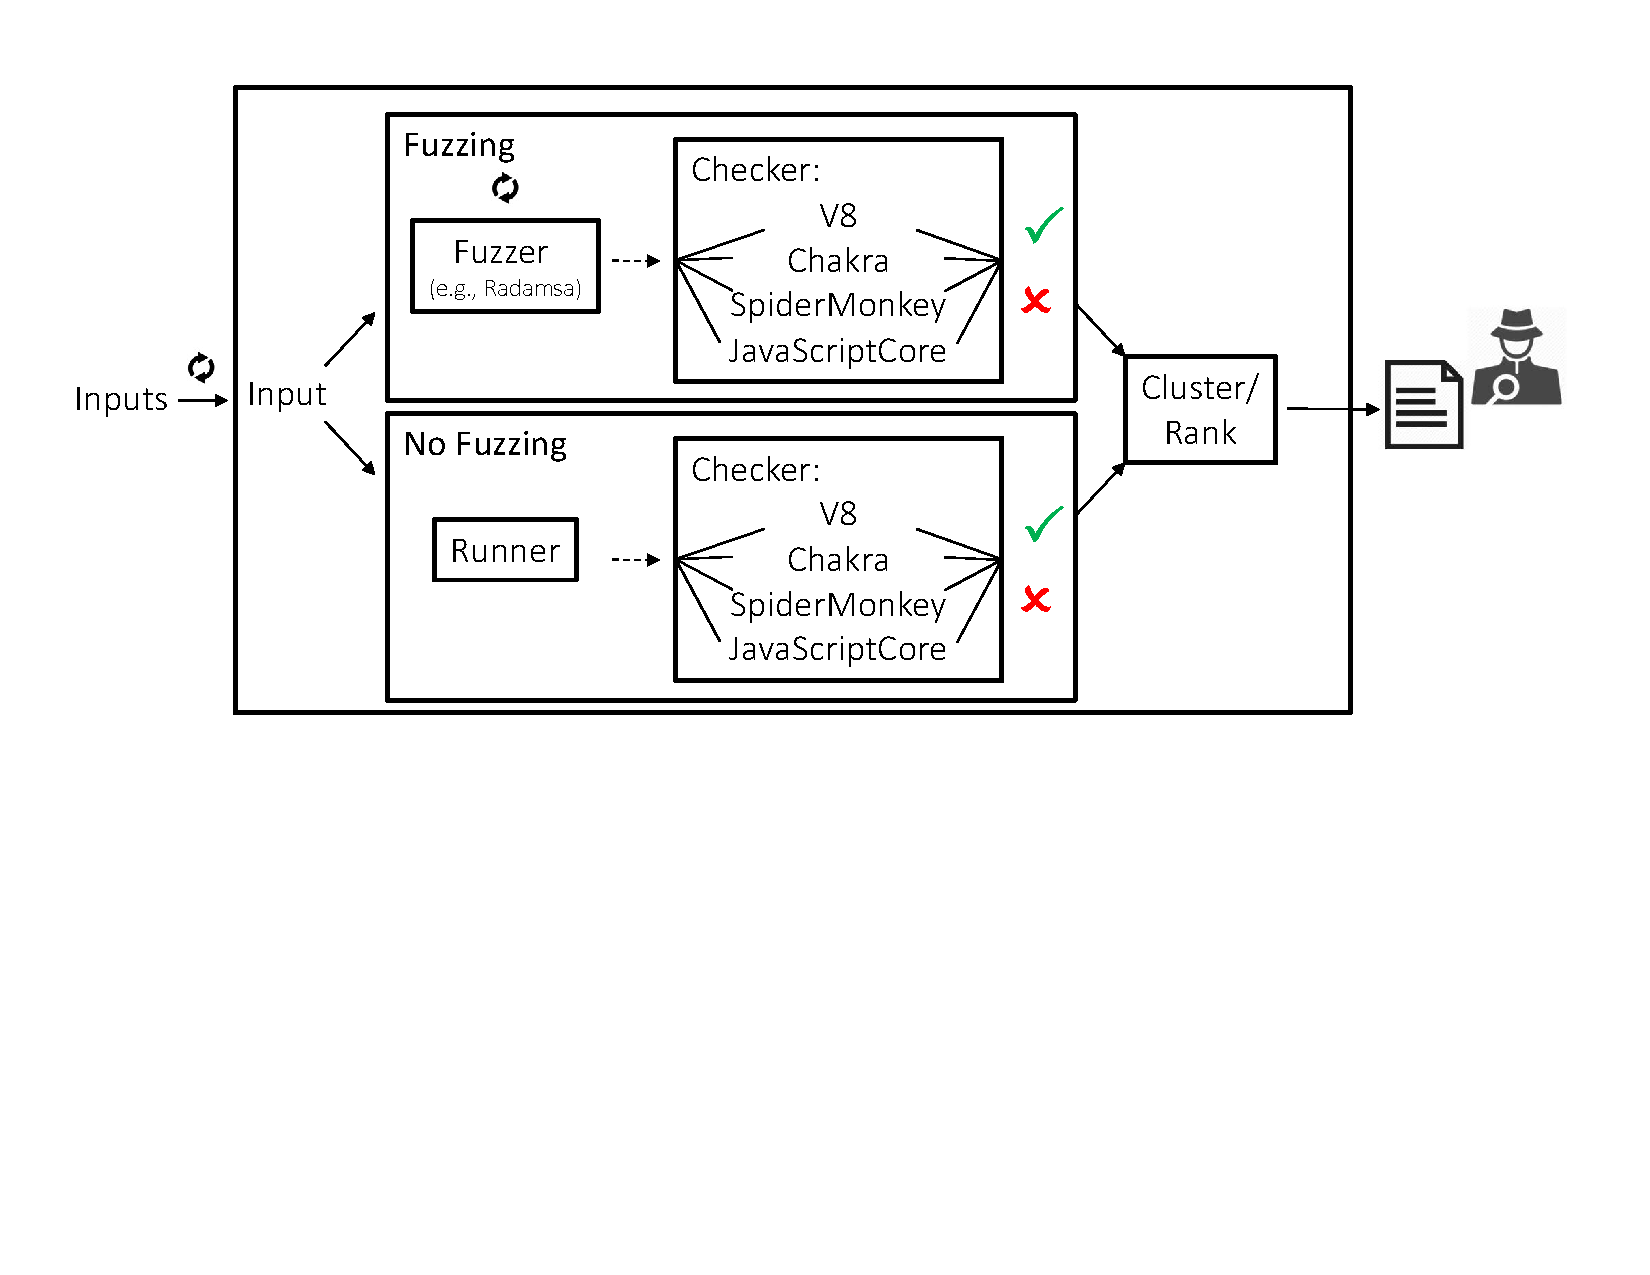
\includegraphics[trim=20 350 200
%    0,clip,width=0.35\textwidth]{google-awards-workflow}
  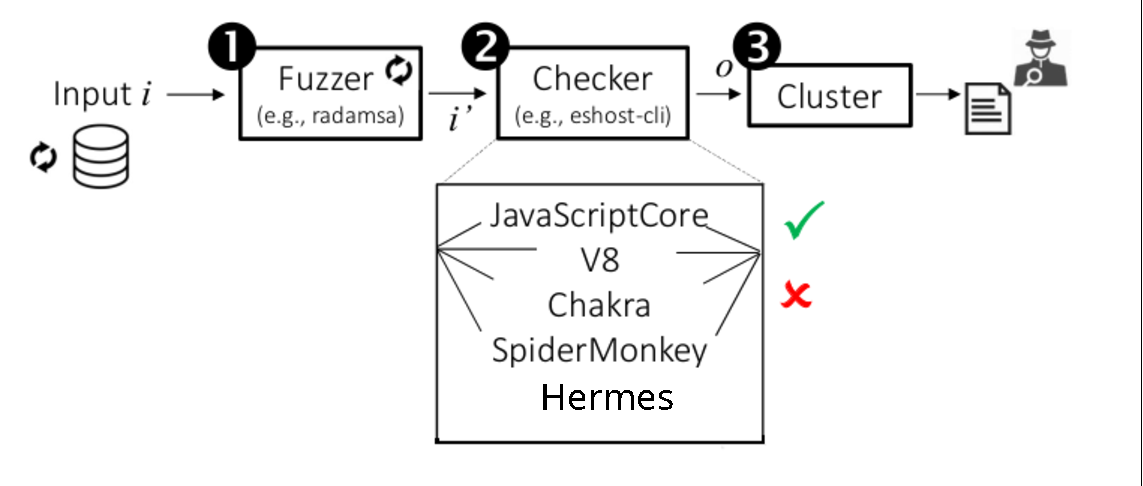
\includegraphics[trim=0 350 0 0,clip,width=0.65\textwidth]{diff-testing-runtimes}
  \caption{\label{fig:workflow}Differential Testing infrastructure overview.}
\end{figure}

The bug-finding process works as follows. New inputs are obtained for
a given test input using some off-the-shelf input
fuzzer~\cite{fuzz-testing-history}.\Comment{ Several fuzzing methods
  have been proposed in the past, varying with respect to how new
  inputs are
  generated~\cite{afl,honggfuzz,grammarinator,jsfunfuzz,radamsa}.}
Section~\ref{sec:objects:fuzzers} describes the fuzzers we selected.
The oracle checks whether or not the output produced for the fuzzed
file is consistent across all engines. In case the test passes in all
engines or fails in all engines (\ie{}, the output is consistent), the
infrastructure discards the test. Otherwise, it considers the input as
potentially fault-revealing; hence interesting for human
inspection. Note that a number of reasons exist, other than a bug, to
explain discrepancy (see Table~\ref{tab:false-positives}). We used the
open-source eshost-cli project~\cite{eshost-cli}, also used at
Microsoft, for checking output discrepancy.

%The checker can produce multiple warnings for a given input. 

Recall that a warning can be manifested for reasons other than a bug
and there is no clear way to distinguish those cases automatically (see
Table~\ref{tab:false-positives}). A human needs to inspect the warning
to diagnose the discrepancy. To facilitate inspection, the
infrastructure prioritize these warnings and clusters them in
groups. Considering prioritization, we classified warnings in two
kinds, reflecting their likelihood to manifest a real bug. Warnings of
the kind ``\hi{}'' are associated with the cases where the test code
executed to completion without violating any internal checks but it
violated assertions declared in the test itself or its harness. The
rationale is that the input is valid--considering the checks declared
in the API functions--but, still, it manifests discrepancy through
violation of an assertion declared in the test.\Mar{example!} In contrast, warnings
in the ``\lo{}'' group reflect the cases where the anomaly was
observed during the execution of functions not related to the test
itself. We found that different engines often check pre-conditions of
those functions differently. It can happen, for example, that one
engine enforces a weaker pre-condition on a function input compared to
another engine and that is acceptable.\Mar{example!} In those cases, our infrastructure would
observe a discrepancy that is more likely to be associated with an
invalid input produced by the fuzzer, \ie{}, it is likely to be a bug
in the test code not the engine (library or runtime) code. Although we
did find real bugs from ``\lo{}'' warnings, the proportion was much
lower compared to ``\hi{}'' warnings. Overall, only \Fix{12\%} of the
reals bugs we found originated from ``\lo{}'' warnings.

\Mar{explain what is a bucket (we refer to it later).} 

\section{Results}
\label{sec:results}

The goal of our study is to assess reliability of \js\ engines by
leveraging implementation diversity, which is specially rich in this
domain. We report results in three parts. First, we report on the
stability of the engines we analyzed using the Test262 standard
conformance test suite for EcmaScript~\cite{ecma262-conformance-suite}
(Section~\ref{sec:stability}). The intuition is that the bugs we
discover throughout this study would have low relevance if the engines
are too fragile. Second, we report results obtained with test
transplantation (Section~\ref{sec:transplantation}). The rationale is
that the domain of possible inputs is too large; consequently, we
expect that test suites written for a given engine cover scenarios and
corner cases uncovered by another engine. To sum, we hope that that
test cases written for one engine could reveal bugs in different
engines as opposed to only manifesting false alarms such as those that
could emerge from implementation-dependent behavior. Third, we
analyzed the impact of using cross-engine differential testing to find
bugs (Section~\ref{sec:cross-engine-diff-testing-results}). The
rationale is that even black-box fuzzers that typically make valid
changes only in literals of the language could expose important
bugs. All in all, we want to assess the impact of simple approaches
that leverage on diversity to find bugs in \js\ engines with the goal
of assessing their reliability.

\subsection{Stability of Engines}
\label{sec:stability}

We evaluated stability with Test262~\cite{ecma262-conformance-suite},
the official \js{} conformance test suite for the ECMA262
specification. We ran this suite once a day for seven consecutive
days. Table~\ref{tab:test262} shows the number of failures over this
period. It is important to note that failures are expected as it takes
time for engines to adjust to the spec. It is also important to
highlight that all engines we analyzed, but \chakra{}, use some
variant of the Test262 suite as part of their regression
process\Mar{with fewer tests?}. We used the official version
instead\Mar{, which updates tests regularly?}. To sum, we observed
that \Fix{...} \Mar{justify regressions using the Kangax report}

\begin{table}[h]
  \centering
  \caption{\label{tab:test262}Number of failures in Test262 over
    a 7-day period.}
  \begin{tabular}{crrrrrrr}
    \toprule
    engine\textbackslash{}day& 1 & 2 & 3 & 4 & 5 & 6 & 7 \\
    \midrule
    \jsc{} & 4330 & 4330 & 4330 & - & - & - & - \\
    \veight{} & 3404 & 3404 & 3401 & - & - & - & - \\
    \chakra{} & 9104 & 9104 & 9104 & - & - & - & - \\
    \smonkey{} & 3943 & 3943 & 3943 & - & - & - & - \\
    \bottomrule 
  \end{tabular}
\end{table}



\subsection{Test Transplantation}
\label{sec:transplantation}

\Mar{remember to say that we use dataset Table II''compile-in-all''.}

This section reports the results of test transplantation, \ie{}, we
analyzed the failures observed when running a test suite on an engine
other than the engine where the test suite
originated.

Table~\ref{tab:cross-testing} shows the number of failures for each
pair of test suite and engine. The first column shows the test suites
and the first row shows the engines that run those tests. We use a
dash (``-'') to indicate that we did not consider the combinations
that associated a test suite with its parent engine; failures in those
cases would either indicate regressions or flaky tests as opposed to
an unknown bug for that engine. We did not run the test cases that
fail on its parent engine in any other engines; we wanted all tests to
pass on their parent engine as a failure in that case would be a
stronger indicative of a bug. In total, 64 test cases were discarded
for that reason--6 from \jsc{} and 58 from \smonkey. In total, 7,029
test files (\ie{}, 38369-31276-64) were considered in this experiment,
which involved 24,922 test runs (\ie, (7029*4)-1021-57-2116).  Of
these, 812 failures were observed (3.25\% of the runs) across
\textbf{543} distinct files (7.72\% of the files). We analyzed each of
these file in separate to identify if the failure was fault-revealing
or a false positive.

We observed from the table that, considering this dataset, the Mozilla
\smonkey\ was the engine that failed the least whereas the Microsoft
engine \chakra\ failed the most. The \smonkey\ test suite also
revealed more failures than any other, perhaps as expected,
considering that it is the suite with more tests (see
Table~\ref{tab:test-suites}).

%% This suggests that the investiment in
%% testing paid off in this case.

\begin{table}[h]
  \centering
  \caption{\label{tab:cross-testing}Number of failures observed exchanging
  test suites.}
  \begin{tabular}{crrrr}
    \toprule
    test suite\textbackslash{}engine & \jsc{} & \veight{} & \smonkey{} & \chakra{}\\
    \midrule
    % \Fix{Versions (03.08)} & 234555 & 7.0.158 & 62.0b14 & 1.10.1 \\
    \Comment{
      Lembrar dos testes que os testes da propria engine falham:
      V8 0 
      JSC 2 
      Spidermonkey 58
    }
    \jsc{} & - & 9 & 10 & 58   \\
    \veight{} & 29 & - & 0 & 0  \\
%    \chakra{} & - & - & - & -  \\
    \smonkey{} & 218 & 107 & - & 279 \\
    Duktape & 0 & 4 & 4 & 1   \\
    \jerry{} & 23 & 25 & 22 & 23   \\
    JSI & 0 & 0 & 0 & 0   \\
    Tiny-js & 0 & 0 & 0 & 0  \\
    \midrule
   \textbf{total} & 270 & 145 & 36 & 361 \\
    \bottomrule 
  \end{tabular}
\end{table}

The piecharts from Figure~\ref{fig:piecharts-transplantation} show the
false and true positives observed with test transplantation. The top
piechart shows false alarms, which means that all
``transplanted'' tests should have passed in these cases. The absolute
number of tests in each category is shown in parentheses to the
right-side of each slice label, naming the source of false
positive. The sources are as follows:

\begin{itemize}
  \item \textbf{Undefined Behavior.} False positives of this kind are
    manifested when tests cover implementation-dependent behavior, as
    defined in the ECMA262 specification~\cite{ecmas262-spec}. For
    example, one of the tests from \jerry\ uses the function
    \CodeIn{Number.toPrecision([precision])}, which translates a
    number to a string, considering a given number of significant
    digits. The floating-point approximation of the real value is
    implementation-dependent, making the test to pass only in
    \chakra\ for that test. As another example, some tests from
    \Fix{Y} use the implementation-dependent description message\Mar{what is the
      name of the property?} encapsulated in an \CodeIn{Error} object
    in assertions. As such, those tests fail in all engines but \Fix{Y}.

  \item \textbf{Timeout/OME\footnote{ome is for out of memory
      error.}.} False positives of this kind manifest because the
    engine that runs the test does not optimize the code as the
    original engine and that has an effect in the test outcome.  The
    test may fail to finish at the time budget or runs out of
    memory. For example, a test case from \jsc{} defines a function
    with a tail-call recursion. The test fails in all engines but
    \jsc{}, which implements tail-call optimization.

    %% \Igor{
    %%   For example, a testcase from \jsc{} suite explores the tail call
    %%   to optimize the recursion, the test uses a recursive function that
    %%   should be executed multiple times (ie. \mcodeid{1e6}). In this case, 
    %%   only the \jsc{} supports tail-call optimization and the testcase 
    %%   passes without failures. Another case can be found in \jerry{} suite
    %%   that uses a repetition statement to concatenate long strings 
    %%   exponentially, causing an out of memory error. The engines used 
    %%   supports the flags to increase memory, however we prefer to use 
    %%   the default engine build.
    %% }

  \item \textbf{Not implemented.} False positives of this kind
    manifest when a test fails because it covers a function that is
    part of the official spec, but is not implemented in the target
    engine. For example, at the time of writing, \chakra{} does not
    implement by default various properties from the \mcodeid{Symbol}
    object. These properties are only available activating ES6
    experimental mode with the flag \CodeIn{-ES6Experimental}.

  \item \textbf{Unknown.} This category corresponds to the cases we
    were unable to confidently diagnose the failure.

  %% \item \textbf{Error message mismatch.} Test fails because it
  %%   compares an error message, which is not portable across
  %%   engines. For example, \Igor{
  %%     a test from the engine \jsc{} uses an assert function called
  %%     \CodeIn{shouldThrow} that expects an specific error message. In this test, 
  %%     all engines throws the Error as expected, however only the message 
  %%     on \jsc{} engine match with the string expected in the test case.
  %%   }
\end{itemize}  

We observed that the sources of false positives were relatively
uniformly distributed, with the categories ``Unknown'' and
``Undefined'' holding more representation with \Fix{X and Y} reports,
respectively. Considering the true positives, we found a reasonable
number of duplicate reports, but not enough high to justify attempting
to automate the detection of duplicates. Section~\ref{sec:bugs}
exemplifies cases of false and true positives.

\begin{figure}[h]
  \centering
  \subfloat[\label{fig:falsepositives}False Positives]{%
    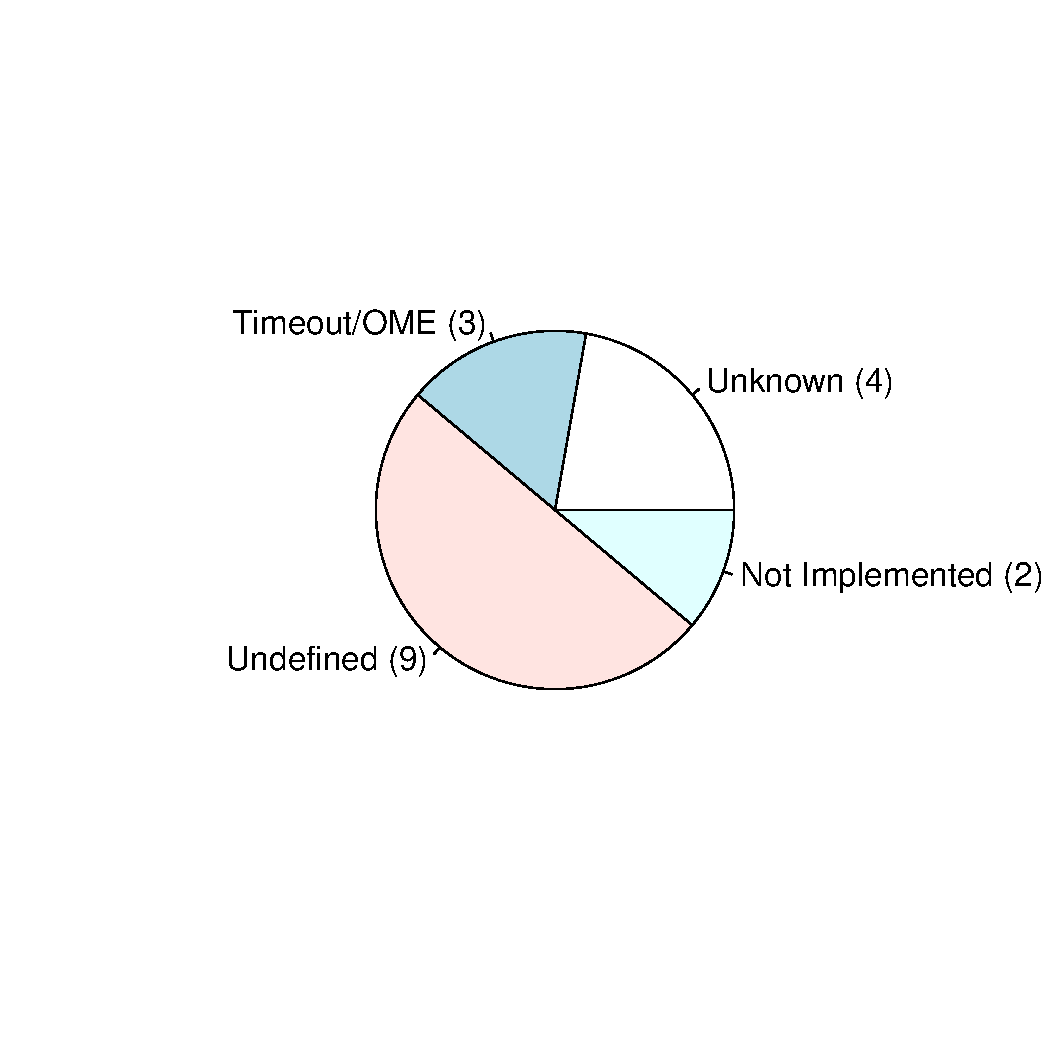
\includegraphics[trim=0 150 0 100,clip,width=0.4\textwidth]{R/piecharts/falsepositives}
  }
  \label{1a}\hfill
  \subfloat[\label{fig:truepositives}True Positives]{%
    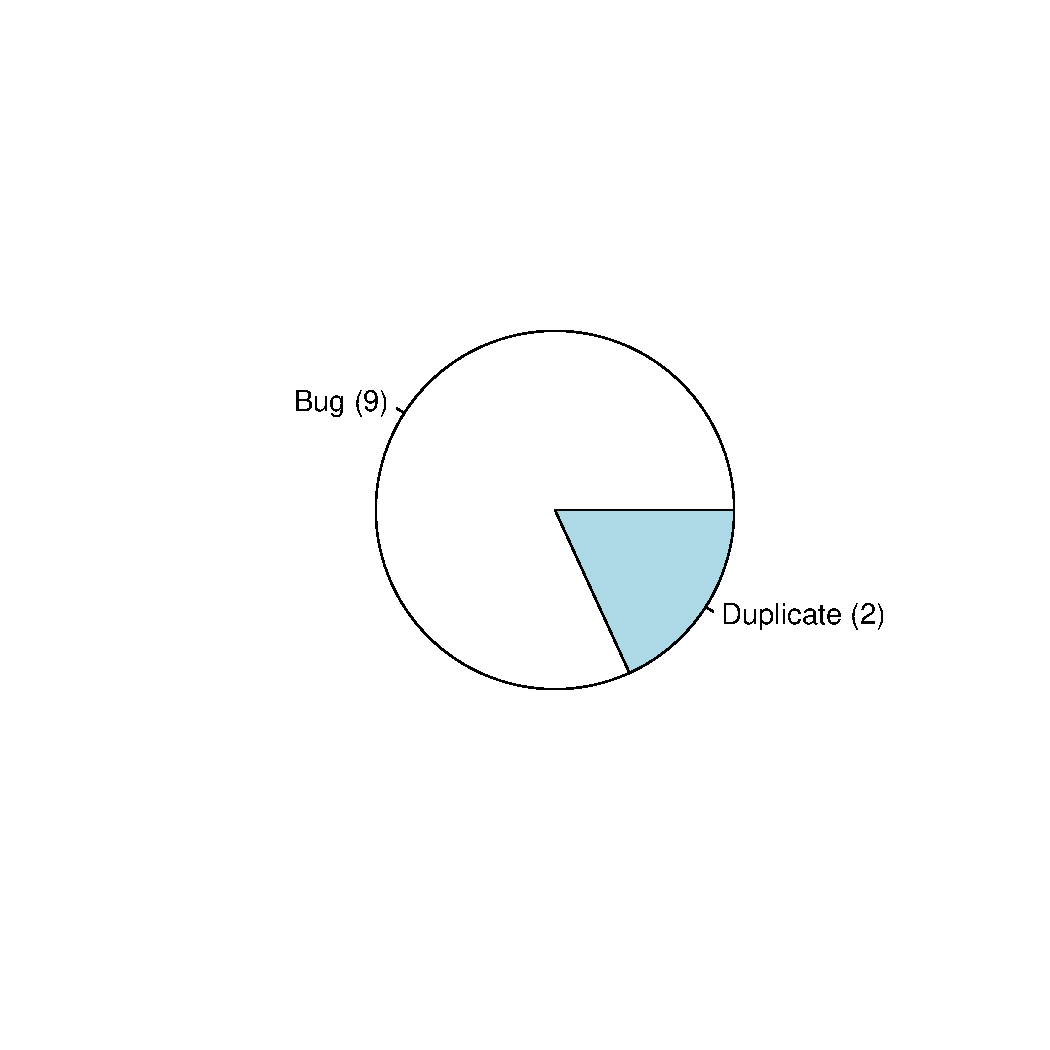
\includegraphics[trim=0 150 0 150,clip,width=0.4\textwidth]{R/piecharts/truepositives}    
  }
  \label{1b}\\
  \caption{\label{fig:piecharts-transplantation}False and True positives.}
\end{figure}

\begin{table*}[t]
  \vspace{-3ex}
%  \scriptsize
  \centering
  \caption{List of bug reports issued as result of test transplantation.}
  \label{tab:test-transplantation-bugs}
  \begin{tabular}{cccccccc}
    \toprule Issue\#    & Date & Engine  & Status  & \multicolumn{1}{c}{Url}  & Severity & Suite \\
    \midrule    
    1  & 4/18  & JavascriptCore  & New  & \anonym{\href{https://bugs.webkit.org/show\_bug.cgi?id=184749}{\#184749}} & - & \jerry{}      \\
   2  & 4/23 & \chakra{}  & \textbf{Confirmed}  & \anonym{\href{https://github.com/Microsoft/\chakra{}Core/issues/5033}{\#5033}} & 2 & \smonkey{}      \\
   3  & 4/29 & \chakra{}  & \textbf{Confirmed}   &
    \anonym{\href{https://github.com/Microsoft/\chakra{}Core/issues/5065}{\#5065}} & 2 & \smonkey{} \\
   \midrule
    \multirow{2}{*}{4}  & \multirow{2}{*}{4/29} & \chakra{} & \textbf{Confirmed} &    \anonym{\href{https://github.com/Microsoft/\chakra{}Core/issues/5067}{\#5067}} & 2 & \multirow{2}{*}{\smonkey{}}\\
                       &  &
    JavascriptCore & New &    \anonym{\href{https://bugs.webkit.org/show\_bug.cgi?id=185130}{\#185130} } &  -  & \\
   \midrule
   5 & 5/02  & JavascriptCore & New  & \anonym{\href{https://bugs.webkit.org/show\_bug.cgi?id=185208}{\#185208}} & - & \smonkey{} \\
   6 & 5/17  & \chakra{} & \textbf{Confirmed} & \anonym{\href{https://github.com/Microsoft/\chakra{}Core/issues/5187}{\#5187}} & 2 & \jsc{}\\
   7 & 5/21  & \chakra{} & \textbf{Confirmed} & \anonym{\href{https://github.com/Microsoft/\chakra{}Core/issues/5203}{\#5203}} & 2 & \smonkey{}\\
   8 & 6/28  & \chakra{} & \textbf{Confirmed}  & \anonym{\href{https://github.com/Microsoft/\chakra{}Core/issues/5388}{\#5388}} & 2 & \jsc{}\\
   9 & 7/10  & \chakra{} & \textbf{Confirmed} & \anonym{\href{https://github.com/Microsoft/\chakra{}Core/issues/5442}{\#5442}} & 2 & \jerry{}\\
   10 & 7/18  & \chakra{} & \textbf{Fixed} & \anonym{\href{https://github.com/Microsoft/\chakra{}Core/issues/5478}{\#5478}} & 2 & \smonkey{}\\
   11 & 7/18  & JavascriptCore & New & \anonym{\href{https://bugs.webkit.org/show_bug.cgi?id=187777}{\#187777}} & - & \jerry{}\\
   12 & 8/07  & \chakra{} & New & \anonym{\href{https://github.com/Microsoft/\chakra{}Core/issues/5576}{\#5576}} & - & \jerry{}\\
   13 & 8/07  & JavascriptCore & \textbf{Fixed} & \anonym{\href{https://bugs.webkit.org/show_bug.cgi?id=188378}{\#188378}} & - & \jerry{}\\
   14 & 8/07  & \chakra{} & New & \anonym{\href{https://github.com/Microsoft/\chakra{}Core/issues/5579}{\#5579}} & - & \jerry{}\\
   15 & 8/07  & JavascriptCore & \textbf{Fixed} & \anonym{\href{https://bugs.webkit.org/show_bug.cgi?id=188382}{\#188382}} & - & \jerry{}\\
   16 & 8/08  & V8 & \textbf{Assigned} & \anonym{\href{https://bugs.chromium.org/p/v8/issues/detail?id=8033}{\#8033}} & 3 & \jerry{}\\
   17 & 8/08  & JavascriptCore & New & \anonym{\href{https://bugs.webkit.org/show_bug.cgi?id=188407}{\#188407}} & - & \jerry{}\\
   \bottomrule
  \end{tabular}
\end{table*}

Figure~\ref{tab:test-transplantation-bugs} lists all bugs we found
with test transplantation. The first column shows the identifier we
assigned to the bug, column ``Date'' shows the date the bug was
reported in the format ``m/dd'', column ``Engine'' shows the affected
engine, column ``Status'' indicates the status of the bug report at
the time of the writing (\eg{},``New'', ``Rejected'', ``Confirmed'',
''Fixed''), column ``Url'' shows the web address for the corresponding
post in the bug tracking system where the discussion thread with
engine developers can be found (de-anonymized upon request), column
``Severity'' shows the severity level for confirmed bugs, and,
finally, column ``Suite'' shows the name of the engine that originated
the test. Considering severity levels, it is important to note that
\jsc{} uses five different severity levels~\cite{jsc-severity} whereas
\chakra{}~\cite{chakra-severity} and \smonkey{}~\cite{mozilla-severity}
use only two. As usual, the smallest the severity value the highest
the severity of the bug. We use a dash (``-'') as the severity level
for bugs with pending confirmation.

Of the \Fix{17} bugs we reported with test transplantation, \Fix{9}
were analyzed and moved from the status ``New'' to ``Confirmed''
(\ie{}, no bug we reported was rejected). Of these, \Fix{8} of them
are severity-2 bugs.  \chakra{} was the engine with the highest number
of confirmed bugs, \Fix{8} in total, with \Fix{1} bug
fixed. Considering the remaining engines, \veight{} confirmed one
bug. Curiously, Google engineers confirmed that report in a few
hours. Although we did not find any showstopper critical bugs, most of
the bugs are seemingly important as per the categorization given by
engineers. Analyzing the issue tracker of \chakra, we found that
severity-1 bugs are rare.


\subsection{Cross-Engine Differential Testing}
\label{sec:cross-engine-diff-testing-results}

This section reports the results obtained by fuzzing inputs, running
those inputs on different engines, and checking the outcomes with a
differential oracle (see Figure~\ref{fig:workflow}). 

\subsubsection{Methodology}
In the following, we describe the methodology we used to assess the
impact of cross-engine differential testing in finding bugs on \js{}
engines. To avoid experimental noise, we did \emph{not} fuzz test
files that failed in some engine as per results reported in
Sections~\ref{sec:stability} and~\ref{sec:transplantation}. The
intuition is that we want to make sure that the bug was not
coincidental, \ie{}, the scenario where fuzzing produces an
fault-revealing input based on a test that was already
fault-revealing. That decision ensures that we can establish
cause-effect relationship between fuzzing and the observation of
discrepancy. For that reason, we discarded a total of \Fix{???} test
files from a total of \totalTestFiles{}.Recall that our tool outputs a
set of buckets, that each bucket includes a set of warnings, that each
warning is related to one file, and that a bucket is of ``lo'' or
``hi'' importance, according to the heuristic we
defined. Figure~\ref{fig:distribution} shows the distribution of
number of warnings reported per bucket. We use the names of the
fuzzing tools to refer to the results obtained with those tools. We
inspected each and every bucket for bugs, but observe that the number
of files per bucket is very high in some cases. As such, it would be
impractical to manually inspect all the files in the bucket. For that
reason, we only inspected one file per bucket. For the cases we found
the warning suspicious, we analyzed the parts of the documentation
related to the problem and, if still suspicious, we looked on the bug
tracker of the affected engine for potential duplicates. If none was
reported, we filed a bug report including the test input that
manifested the potential problem and explaining the reasons we were
suspicious. In some cases, we used the Mozilla lithium
tool~\cite{lithium} to minimize the test case. For the cases of false
positives, we identified the source of false positive and moved to the
next bucket.


\begin{figure}[t]
  \centering
  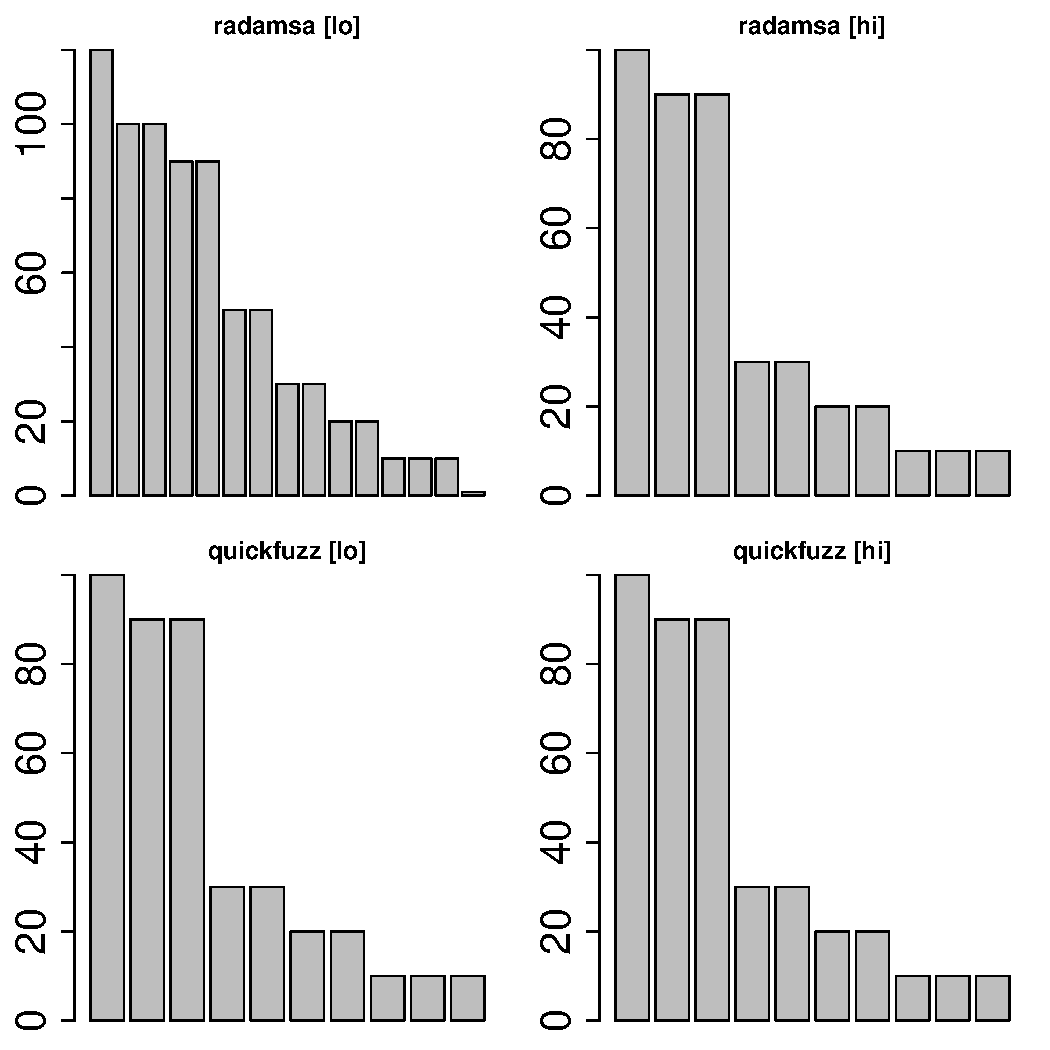
\includegraphics[trim=0 0 0 0,clip,width=0.40\textwidth]{R/histograms/histograms.pdf}  
  \caption{\label{fig:distribution}Distribution of lo and hi warnings
   in buckets.}
\end{figure}


\subsubsection{Results}
Table~\ref{tab:summary-of-results} summarizes our results. It shows,
for each fuzzer and kind of bucket (\ie{}, hi or lo), the total number
of files involved, the number of buckets reported by our
infrastructure, the number of those that we classified as
bug-revealing (positive), and the number of those that we filed a bug
report. The difference between the last two columns corresponds to the
number of duplicates, \ie{}, the cases of bugs already reported in the
corresponding issue tracker. As expected, the hit ratio for the ``hi''
group is higher, indicating that chances of filing a bug report for a
``hi'' warning is higher.

\begin{table}[h]
  \centering
  \caption{\label{tab:summary-of-results}Summary of results.}
  \begin{tabular}{ccrrrr}
    \toprule
    \multirow{2}{*}{mode} & \multirow{2}{*}{type} & \multirow{2}{*}{\# files} &  \multicolumn{3}{c}{buckets} \\
    \cline{4-6}    
    & & & \multicolumn{1}{c}{\#} & \multicolumn{1}{c}{\# pos.} &
    \multicolumn{1}{c}{\# pos. filed} \\
    \midrule
    %% \multirow{2}{*}{nofuzz} & lo & \nofuzzFilesLO{} &  \nofuzzLOTotal{} & \Fix{.} & 11 (34) \\
    %% & hi & \nofuzzFilesHI{} & \nofuzzHITotal{} & \Fix{.} & \Fix{108 (-)} \\
    \multirow{2}{*}{\radamsa} & lo & \Fix{.} & \Fix{.} & \Fix{.} & \Fix{.} \\
    & hi & \Fix{.} & \Fix{.} & \Fix{.} & \Fix{.} \\
    \multirow{2}{*}{\quickfuzz} & lo & \Fix{.} & \Fix{.} & \Fix{.} & \Fix{.} \\
                             & hi & \Fix{.} & \Fix{.} & \Fix{.} & \Fix{.} \\    
    \bottomrule     
  \end{tabular}
\end{table}

Table~\ref{tab:false-positives} shows the distribution of false
positives per source. A false positive is a bucket that did not lend
itself in a bug report. The sources of imprecision are as defined in
Section~\ref{sec:transplantation} with the addition of two new
sources, which we did not observe before. The source ``Invalid Input''
indicates that the test violated some part of the specification. For
example, the test indirectly invoked some function with unexpected
arguments\Fix{provide concrete example}. The source ``Upcoming
Feature'' indicates that the test fails because it uses a feature that
is available in the original engine, but it is still not standard, and
the target engine does not support that feature. For example,
\Fix{provide concrete example} 

\begin{table}[t]
  \centering
  \caption{\label{tab:false-positives}Distribution of false
    positives buckets per source.}
  \begin{tabular}{crr}
    \toprule
    & \radamsa\ & \quickfuzz\ \\
    Undefined & - & - \\
    Timeout/OME & - & - \\
    Not Implemented & - & - \\
    Upcoming Feature & - & - \\
    Error Message Mismatch & - & - \\    
    Invalid Input & - & - \\    
    \bottomrule     
  \end{tabular}
\end{table}

% \Igor{
%   Para realizar nossos experimentos, tivemos que decidir qual as 
%   melhores abordagens para aumentar a efetividade dos fuzzers.
%   Os fuzzers mutacionais se mostraram mais eficientes em relacao
%   aos fuzzers geracionais, entao focamos neste ponto.
%   Utilizamos os fuzzers radamsa, QuickFuzz e \Fix{others} nas suas configuracoes
%   default para realizar a mutacao em arquivos existentes.
%   O fuzzer radamsa eh um fuzzer mutacional agnostico de linguagem e possui algumas
%   deficiencias para a nossa infraestrutura como a falta de uma gramatica para guiar a suas mutacoes, 
%   pois muitas das vezes a unica mutacao ocorre em uma palavra dentro de um comentario por exemplo.
%   O fuzzer QuickFuzz tem uma gramatica JS integrada e sua mutacao ocorre de forma mais robusta que o 
%   radamsa, gerando arquivos mais relevantes.
%   Nossa infraestrutura usa a library Esprima\footnote{cite esprima url} para garantir que o arquivo fuzzado
%   é um arquivo de teste relevante, seguindo estes requisitos:
%   \begin{itemize}
%     \item it contains only unicode text
%     \item it is parseable (i.e., it is structurally well-formed)
%     \item it does not contain engine-specific functions  
%     \item it does not empty
%   \end{itemize}

% }

\section{Bugs Found}
\label{sec:bugs}

%% Although there are many features yet to implement in our
%% infrastructure,

\begin{table*}[h!]
  \vspace{-3ex}
%  \scriptsize
  \centering
  \caption{List of bug reports issued as result of cross-engine
    differential testing.}
  \label{tab:bugs}
  \begin{tabular}{ccccccccc}
    \toprule
    Issue\#    & Date & Fuzz & Engine  & Status  &
    \multicolumn{1}{c}{Url}  & Severity & Priority & Suite \\
    \midrule    
    1  & 4/12 & radamsa & \chakra{}   & \textbf{Fixed}  &
    \anonym{\href{https://github.com/Microsoft/\chakra{}Core/issues/4978}{\#4978}}
    & 2 & LO & \jsc{} \\ 
    2  & 4/12 & radamsa & \chakra{}   & Rejected  &
    \anonym{\href{https://github.com/Microsoft/\chakra{}Core/issues/4979}{\#4979}}
    & - & HI & \jsc{} \\
    3  & 4/14 & radamsa & JavascriptCore  & New &
    \anonym{\href{https://bugs.webkit.org/show\_bug.cgi?id=184629}{\#184629}
    } & -  & HI & \jsc{}    \\
    4  & 4/25 & radamsa & \chakra{}  & \textbf{Fixed}     &
    \anonym{\href{https://github.com/Microsoft/\chakra{}Core/issues/5038}{\#5038}}
    & 2 & HI & \jerry{}   \\
    5  & 4/29 & radamsa & JavascriptCore  & New  &
    \anonym{\href{https://bugs.webkit.org/show\_bug.cgi?id=185127}{\#185127}
    } & -  & HI  & \jerry{}\\
    \midrule
    \multirow{2}{*}{6} & \multirow{2}{*}{4/30}  &
    \multirow{2}{*}{radamsa} & \chakra{} & \textbf{Confirmed} &
    \anonym{\href{https://github.com/Microsoft/\chakra{}Core/issues/5076}{\#5076}}
    & 2 & \multirow{2}{*}{HI} & \multirow{2}{*}{TinyJS}\\    
                        &                        &        &
    JavascriptCore & New &
    \anonym{\href{https://bugs.webkit.org/show\_bug.cgi?id=185156}{\#185156}}
    & - &  & \\
    \midrule
    7 & 5/02 & radamsa & JavascriptCore  & \textbf{Fixed} &
    \anonym{\href{https://bugs.webkit.org/show\_bug.cgi?id=185197}{\#185197}}
    & 2 & LO & \smonkey{} \\
    8 & 5/10 & radamsa & \chakra{} & \textbf{Confirmed} &
    \anonym{\href{https://github.com/Microsoft/\chakra{}Core/issues/5128}{\#5128}}
    & 3 & HI & \jerry{} \\
    9 & 5/17 & radamsa & \chakra{} & \textbf{Fixed} &
    \anonym{\href{https://github.com/Microsoft/\chakra{}Core/issues/5182}{\#5182}}
    & 2 & HI & \veight{}\\
    10 & 5/24 & radamsa & JavascriptCore & \textbf{Fixed}  &
    \anonym{\href{https://bugs.webkit.org/show\_bug.cgi?id=185943}{\#185943}}
    & 2 & HI & \jsc{}\\
    11 & 6/26 & radamsa & JavascriptCore & \textbf{Fixed}  &
    \anonym{\href{https://bugs.webkit.org/show_bug.cgi?id=187042}{\#187042}}
    & 2 & HI & \jerry{}\\
    12 & 7/10 & quickfuzz & \jsc{} & \textbf{Fixed}  &
    \anonym{\href{https://bugs.webkit.org/show_bug.cgi?id=187520}{\#187520}}
    & 2 & HI & \jerry{}\\
    13 & 7/10 & quickfuzz & \chakra{} & \textbf{Confirmed}  &
    \anonym{\href{https://github.com/Microsoft/\chakra{}Core/issues/5443}{\#5443}}
    & 2 & HI & \jerry{}\\
   \bottomrule
  \end{tabular}
\end{table*}


This section shows results obtained with our
infrastructure. Table~\ref{tab:bugs} shows the list of bugs we
reported on issue trackers of different engines in the period of 42
days. So far, ten of the bugs we reported
were confirmed, two of which were fixed. One bug report we
submitted was rejected on the basis that the offending JS file
manifested an expected incompatibility across engine
implementations.
Note from the table that all bug
reports still waiting for confirmation are associated with the
\jsc{} engine (JSC). A closer look at the JSC issue tracker
showed that the triage process is very slow for that engine. 
\Igor{
The bugs reported on \chakra{}'s bug tracker was defined as confirmed, 
however the bugs are included on a milestone for the next release
following an internal priority.
}
As of now, we did not find any new bug on \smonkey{} and V8; 
the bugs we found were duplicates and were not reported. Finally, it is
worth noting that \Fix{11 of the 19} JS files that manifested
discrepancies were \emph{not} produced with fuzzing (column
``Fuzz''). These are test files from suites of different engines. This
observation emphasizes the importance of continuously collecting test suites from
multiple sources; today, we use test suites from seven different open
source engines, including a total of 30K test files.

\Mar{justify why we discuss these bugs} \Mar{discuss other bugs}

\vspace{1ex}\noindent\textbf{Bug \# 6.} The JS code \CodeIn{var a = \{valueOf:~function()\{return
  ``\textbackslash{}x00''\}\} assert(+a === 0)\}} 
manifested a bug in the \js{} engine \chakra{}.  The object
property \CodeIn{valueOf} stores a function that returns a primitive
value identifying the target object~\cite{valueof}. The original
version of this code returns an empty string whereas the version of
the code modified by the Radamsa fuzzer~\cite{radamsa} returns a string
representation of a null character (called \CodeIn{NUL} in ascii). The
unary plus expression ``\CodeIn{+a}", appearing in the assertion, is
equivalent to the abstract operation \CodeIn{ToNumber(a.valueOf())}
that converts a string to a number, otherwise the operation returns
NaN (Not a Number)\cite{unary-plus}. For this case, \chakra{} evaluates
the unary plus to NaN as expected, as the null character cannot be
converted. As result, the test fails as expected. \chakra{}, in contrast,
incorrectly converts the string to zero, making the test to pass. All
other engines fail on this test. As Table~\ref{tab:bugs} shows, the
\chakra{} team fixed the issue soon after we reported the problem.

\subsection{False Positives}

An example of a warning from the HI group is defined in Figure~\ref{fig:hi-priority}. 
This is a testcase from WebKit.es6 suite that it was mutate by radamsa fuzzer, the 
initial seed has in line 3 the code \CodeIn{"foo".repeat(3)} but the fuzzer changed the 
integer 3 to a big integer number. We reported this case in \chakra{} due a core dumps that occurs
during the runtime, however this case was rejected due \CodeIn{incompatibility by design} that
this is an intentional behavior of engine that crash the process if it runs out of memory.

\begin{figure}[h!]
  \centering
  \scriptsize
  \lstset{escapeinside={@}{@},
    numbers=left,xleftmargin=1em,frame=single,framexleftmargin=0.5em,
    basicstyle=\ttfamily\scriptsize, boxpos=c,
    numberstyle=\tiny,
    morekeywords={assertEq, var, yield, in, function, 
    typeof, return, throw, new, Error, if},
  }
  \begin{lstlisting}
function test() {
  return typeof String.prototype.repeat === "function"
    && "foo".repeat(657604378) === "foofoofoo";
}
if (!test())
  throw new Error("Test failed");
  \end{lstlisting}
  \normalsize
  \caption{Warning captured as HI priority.}
  \label{fig:hi-priority}
  \end{figure}

% \subsection{LO bugs}
% 
% \Igor{For example, a bug caught by our environment and reported as LO priority was reported 
% on \chakra{} engine, the JS code can be found in Figure~\ref{fig:lo-priority}. In this case,
% this is a seed from Mozilla suite (\CodeIn{mozilla/non262/statements/for-in-with-assignments.js}),
% the warning was not caught by the \CodeIn{assertEq} function that compares if two arguments are equals, 
% the bug appears inside the generator function\footnote{Generators \url{https://developer.mozilla.org/en-US/docs/Web/JavaScript/Reference/Statements/function*}}
% at line 2. According to ES6 specification\footnote{ES6 YieldExpression \url{https://www.ecma-international.org/ecma-262/8.0/index.html\#prod-YieldExpression}},
% it is allowed the use of \CodeIn{yield in} in a \CodeIn{for} loop. In our infrastructure,
% only \chakra{} engine fails with an error output \CodeIn{SyntaxError: Syntax error}, due
% the output does not shows nothing related with assertions, we considered this one as a warning from LO group.
% Until now, the issue was confirmed and waiting for merge/closed.
% \Fix{checar ate o prazo de submissao. Essa issue esta confirmada e com commits, falta apenas o merge.}
% }
% \begin{figure}[h!]
%   \centering
%   \scriptsize
%   \lstset{escapeinside={@}{@},
%     numbers=left,xleftmargin=1em,frame=single,framexleftmargin=0.5em,
%     basicstyle=\ttfamily\scriptsize, boxpos=c,
%     numberstyle=\tiny,
%     morekeywords={assertEq, var, yield, in, function},
%   }
%   \begin{lstlisting}
% function* g1() {
%   for (var x = yield in {}) ;
% }
% var it = g1();
% assertEq(it.next().done, false);
% assertEq(it.next().done, true);
%   \end{lstlisting}
%   \normalsize
%   \caption{Bug caught by our environment as LO priority.}
%   \label{fig:lo-priority}
%   \end{figure}

\section{Related Work}

\Fix{The
  closest work to ours was done by Patra and Pradel~\cite{patra2016learning},
  where they evaluated their proposed language-agnostic fuzzer to find
  cross-browser HTML+JS discrepancies. This project aims at building
  and evaluating an infrastructure for differential testing of runtime
  engines, such as the JS engine or WebAssembly's. The sensible parts
  of the infrastructure are the checks of input validity (as to reduce
  waste/cost) and output correctness (as to reduce false positives).}

RFC-Directed Differential Testing of Certificate Validation in SSL/TLS Implementations...[ICSE18]

%\section*{Acknowledgment}

%\bibliographystyle{IEEEtran}
\balance
\bibliographystyle{plain}
\bibliography{references,../docs/google-research-awards-latam/tmp}

\end{document}

%%  LocalWords:  bytecodes JScript Ecma ome IoT Kangax DT JS fuzzer
%%  LocalWords:  jsfunfuzz jit funfuzz \smonkey{} toPrecision JSVU
%%  LocalWords:  GoogleChromeLab's cccr js runtime Fuzzers Radamsa de
%%  LocalWords:  QuickFuzz fuzzers Grammarinator LangFuzz Megadeth
%%  LocalWords:  AFL libFuzzer toolchain sanitizers arrowed eshost
%%  LocalWords:  cli pre EcmaScript dataset piecharts piechart \chakra{}
%%  LocalWords:  JavascriptCore Url radamsa TinyJS \jerry{} JSC
%%  LocalWords:  quickfuzz \jsc{} \chakra{}'s valueOf NUL ascii
%%  LocalWords:  unary ToNumber NaN testcase WebKit typeof foofoofoo
%%  LocalWords:  SSL TLS ICSE
